%%%%%%%%%%%%%%%%%%%%%%%%%%%%%%%%%%%%%%%%%%%%%%%%%%%%%%%%%%%%%%%%%%%%%%%%%%%%%%%%
\section{Shape-from-Shading}\label{ch:bg_sfs}
%%%%%%%%%%%%%%%%%%%%%%%%%%%%%%%%%%%%%%%%%%%%%%%%%%%%%%%%%%%%%%%%%%%%%%%%%%%%%%%%
%%%%%%%%%%%%%%%%%%%%%%%%%%%%%%%%%%%%%%%%
\begin{figure}[t]
	\centering
	\begin{subfigure}[b]{0.24\textwidth}
		\centering
		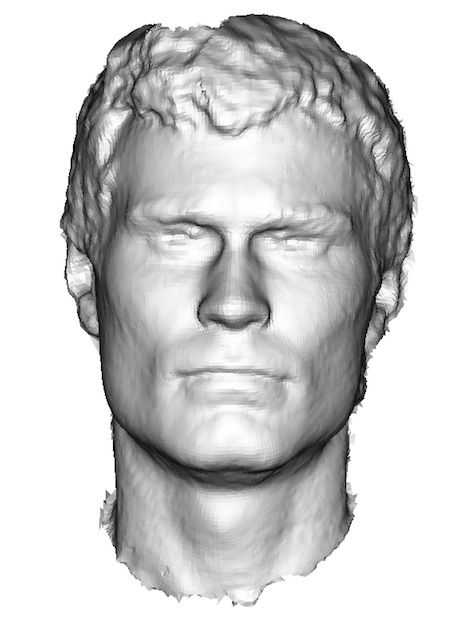
\includegraphics[height=2in]{background/images/frontal}
		\caption*{Frontal}
	\end{subfigure}
	\begin{subfigure}[b]{0.24\textwidth}
		\centering
		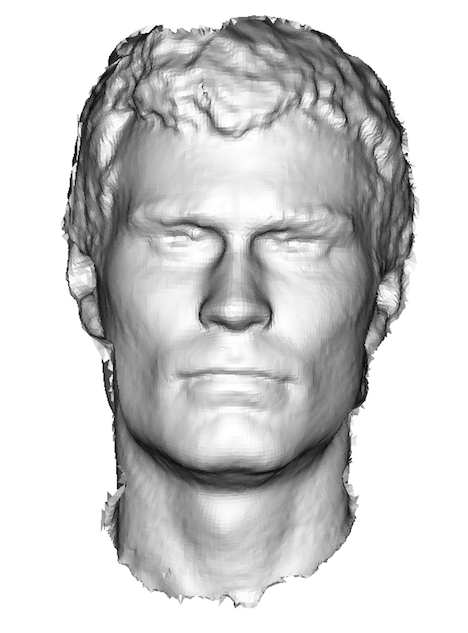
\includegraphics[height=2in]{background/images/invert}
		\caption*{Inverted}
	\end{subfigure}
	\begin{subfigure}[b]{0.24\textwidth}
		\centering
		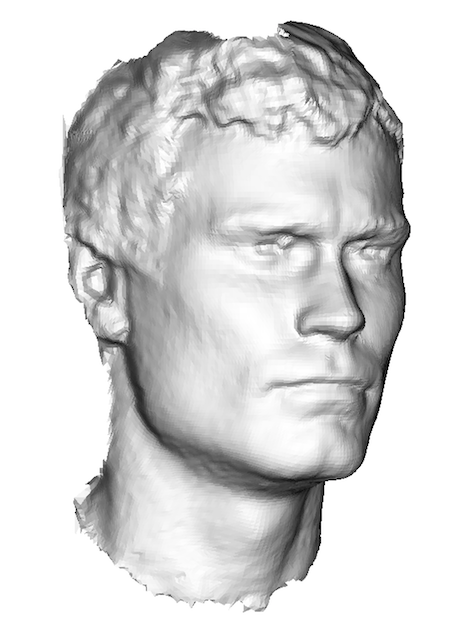
\includegraphics[height=2in]{background/images/frontal_rotate}
		\caption*{Frontal}
	\end{subfigure}
	\begin{subfigure}[b]{0.24\textwidth}
		\centering
		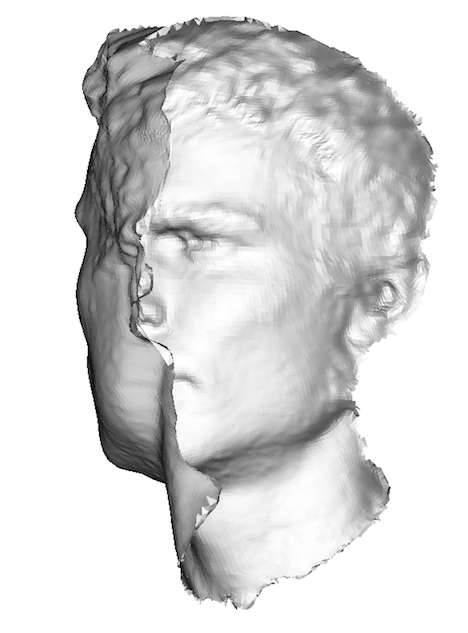
\includegraphics[height=2in]{background/images/invert_rotate}
		\caption*{Inverted}
	\end{subfigure}
	\caption{An example of a bas-relief ambiguity for a mesh illuminated
	         frontally under orthographic projection, with a lambertian shader. 
	         ``Inverted'' implies that the mesh is actually facing away from the
	         camera and thus the interior is visible, as demonstrated by the
	         rotated ``Inverted'' image. Both of the non-frontal images are
	         rotated versions of the frontal images, approximately $25^\circ$
	         around the Yaw axis.}
\label{fig:sfs_bas_relief}
\end{figure}
%%%%%%%%%%%%%%%%%%%%%%%%%%%%%%%%%%%%%%%%
Shape-from-shading (SfS) is the process of attempting to recover surface
information from an object in an image using \textit{inverse rendering}, 
or \textit{image formation}, methods. The primary assumption is that shading, or
the intensity of a pixel in the image, is generated as a function of the surface
geometry and its interaction with light reflected/absorbed by the surface and
captured by an imaging device. Naturally, the reality of this process in the
physical world is a complex interaction between light and both microscopic and
macroscopic elements of the surface structure. This is further complicated by
the noise present in the recording procedure of the camera sensing
hardware. Furthermore, it is well known that shading alone is insufficient to
disambiguate shape. For example, the well known bas-relief
ambiguity~\cite{belhumeur1999bas} is demonstrated for a facial mesh in
\cref{fig:sfs_bas_relief}. The bas-relief ambiguity states that for an object
imaged under orthographic projection that exhibits lambertian reflectance, there
exists a family of transformations (generalized bas-relief transformations) for
which the images produced will be identical. In fact, more generally there
exists an infinite number of ways to describe any image given only shading
information through different arrangements of surfaces, lightings and
albedos~\cite{adelson1996perception}. However, despite the ill-posedness of the
SfS problem, shading does in fact provide a very strong imaging prior and many
higher frequency detail such as wrinkles can only be recovered using shading
cues. Before discussing the facial surface recovery literature, we briefly 
describe the image formation problem including the common assumptions
made.
%%%%%%%%%%%%%%%%%%%%%%%%%%%%%%%%%%%%%%%%%%%%%%%%%%%%%%%%%%%%%%%%%%%%%%%%%%%%%%%%
\subsection{Image Formation}
%%%%%%%%%%%%%%%%%%%%%%%%%%%%%%%%%%%%%%%%%%%%%%%%%%%%%%%%%%%%%%%%%%%%%%%%%%%%%%%%
%%%%%%%%%%%%%%%%%%%%%%%%%%%%%%%%%%%%%%%%
\begin{figure}
	\centering
	\begin{tabular}{cc}
		\multicolumn{2}{c}{
			\begin{subfigure}[b]{\textwidth}
				\centering
				\caption*{Radiometric Terms}
				\begin{tabular}{@{}lll@{}}
					\toprule
					Term              & Symbol                                      & Unit                 \\ \midrule
					Solid Angle       & $d\omega$                                    & ${sr}^{-1}$          \\
					Radiant Flux      & $\Phi$                                       & $W$                  \\
					Radiant Intensity & $J = d \Phi / d \omega$                      & $W {sr}^{-1}$        \\
					Irradiance        & $E = d \Phi / d A$                           & $W m^{-2}$           \\
					Radiance          & $L = d^2 \Phi / (dA \cos{\theta_r} d\omega)$ & $W m^{-2} {sr}^{-1}$ \\ \bottomrule
				\end{tabular}
			\end{subfigure}
		} \\[2cm]
		\begin{subfigure}[b]{0.48\textwidth}
			\centering
			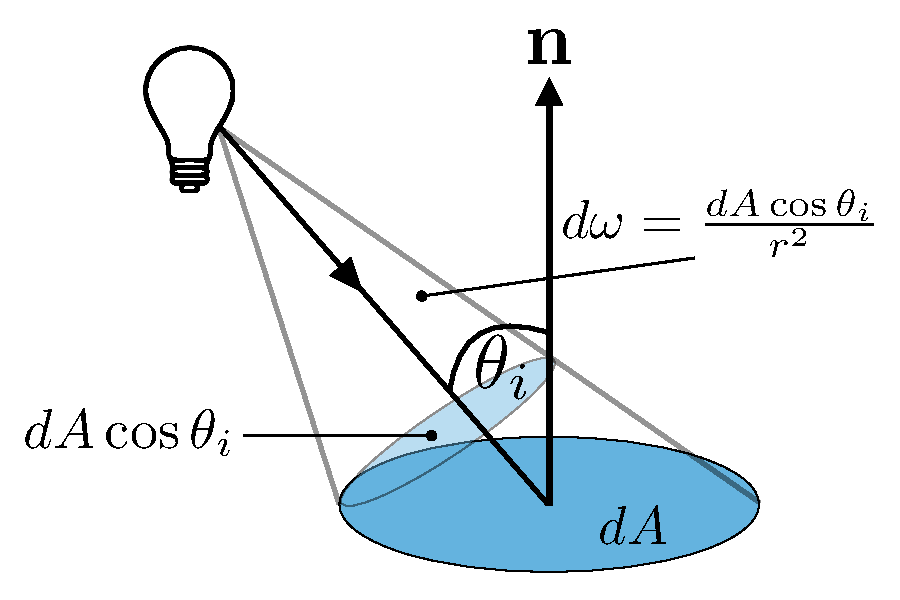
\includegraphics[width=\textwidth]{background/images/irradiance}
			\caption*{Irradiance}
		\end{subfigure} & 
		\begin{subfigure}[b]{0.48\textwidth}
			\centering
			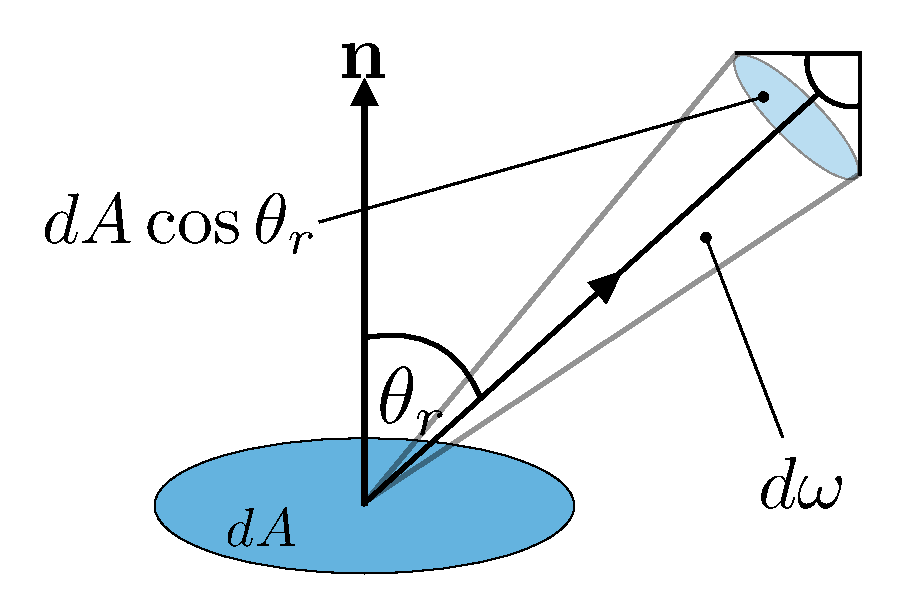
\includegraphics[width=\textwidth]{background/images/radiance}
			\caption*{Radiance}
		\end{subfigure}
	\end{tabular}
	\caption{Illustration of common radiometric terms, focusing on the surface
	         irradiance and radiance. ${sr}^{-1}$ denotes steradians, the 
	         Standard International unit of solid angular measure and
	         $W$ denotes watts.}
\label{fig:bg_sfs_rad_irrad}
\end{figure}
%%%%%%%%%%%%%%%%%%%%%%%%%%%%%%%%%%%%%%%%
When discussing image formation methods a number of assumptions are commonly 
made in order to ensure tractability of of the rendering physics. Firstly,
unless explicitly mentioned, we assume an orthographic camera projection. This
is a reasonable assumption for most facial images as faces tend to the be
the focus of an image and thus photographs are commonly taken close enough
to the face that perspective effects are minimal. We also only consider
reflection functions that can be expressed as a Bidirectional 
Reflectance-Distribution Function (BRDF). A BRDF is a convenient construct
that allows the expression of how bright a surface will appear from a given
view point direction when illuminated from another direction. More formally, it 
is the ratio of the reflected radiance in the viewing direction to the 
irradiance, in the direction toward the light source. 
See \cref{fig:bg_sfs_rad_irrad} for an illustration of the radiance and
irradiance as well as a table of useful radiometric terms.
\textit{Radiant flux} is the power emitted from a light source, measured in 
watts $(W)$.
The \textit{solid angle} subtended by a surface patch is defined as the 
surface area of a unit sphere covered by the surface's projection onto the 
sphere and is measured in steradians $(sr)$. In \cref{fig:bg_sfs_rad_irrad},
$r$ refers to the distance from the sphere's origin to the patch.
\textit{Radiant intensity} is the radiant flux per unit solid angle and is 
measured in watts per steradian $(W {sr}^{-1})$. 
The \textit{irradiance} is the amount of energy received by a given surface
patch, measured in watts per square meter $(W m^{-2})$. 
The \textit{radiance} is the amount of energy emitted per unit foreshortened
surface area per unit solid angle, measured in watts per square meter 
per steradian $(W m^{-2} {sr}^{-1})$. In \cref{fig:bg_sfs_rad_irrad},
the unit foreshortened area is given by $dA \cos{\theta_r}$.
It is important to note that radiance, unlike irradiance, is a directional 
quantity. This implies that the viewing angle affects the amount of perceived
light from a given image area and for some reflectance functions that manifests
as specular style highlights. Finally, we rely on the fact that the image
irradiance captured by the camera sensor is directly proportional to the
scene radiance~\cite{horn1979calculating}. Given the previous notation, we
can now formally define the general equation for a BRDF
%%%%%%%%%%%%%%%%%%%
\begin{align}
	f(\theta_i,\phi_i;\theta_r,\phi_r) &= \frac{L(\theta_r,\phi_r)}{E(\theta_i,\phi_i)} \\
	L(\theta_r,\phi_r)                 &= E(\theta_i,\phi_i) f(\theta_i,\phi_i;\theta_r,\phi_r) \\
	L(\theta_r,\phi_r)                 &= \int_{2\pi} I_{\operatorname{src}}(\theta_i,\phi_i) f(\theta_i,\phi_i;\theta_r,\phi_r) \; \cos{\theta_i} \; d\omega_i
\end{align}
%%%%%%%%%%%%%%%%%%%
$I_{\operatorname{src}}(\theta_i,\phi_i)$ is the intensity of output
from a given light source. In fact, assuming an isotropy, the BRDF is
only a function of 3 parameters, $f(\theta_i,\theta_r, \Delta \phi)$ where
$\Delta \phi = \phi_i - \phi_r$. We also assume Helmholtz reciprocity, which
states that if the light source and viewing direction are swapped the BRDF
remains unchanged 
\ie~$f(\theta_i,\phi_i;\theta_r,\phi_r) = f(\theta_r,\phi_r;\theta_i,\phi_i)$.
An illustration of the general BRDF is given in \cref{fig:sfs_brdf_example}.
%%%%%%%%%%%%%%%%%%%%%%%%%%%%%%%%%%%%%%%%
\begin{figure}[t]
	\centering
	\begin{subfigure}[b]{0.45\textwidth}
		\centering
		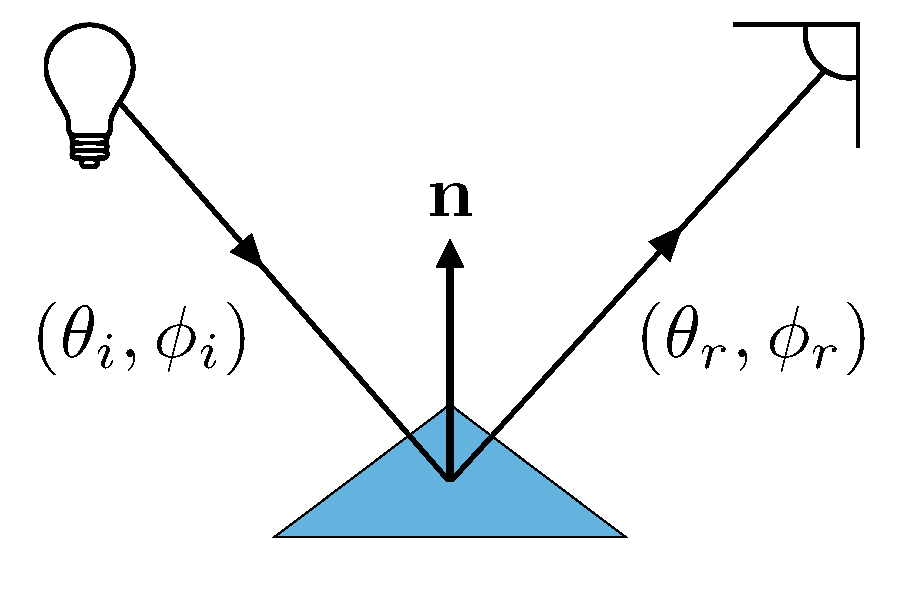
\includegraphics[width=\textwidth]{background/images/general_brdf}
		\caption*{General BRDF}
	\end{subfigure}
	\begin{subfigure}[b]{0.45\textwidth}
		\centering
		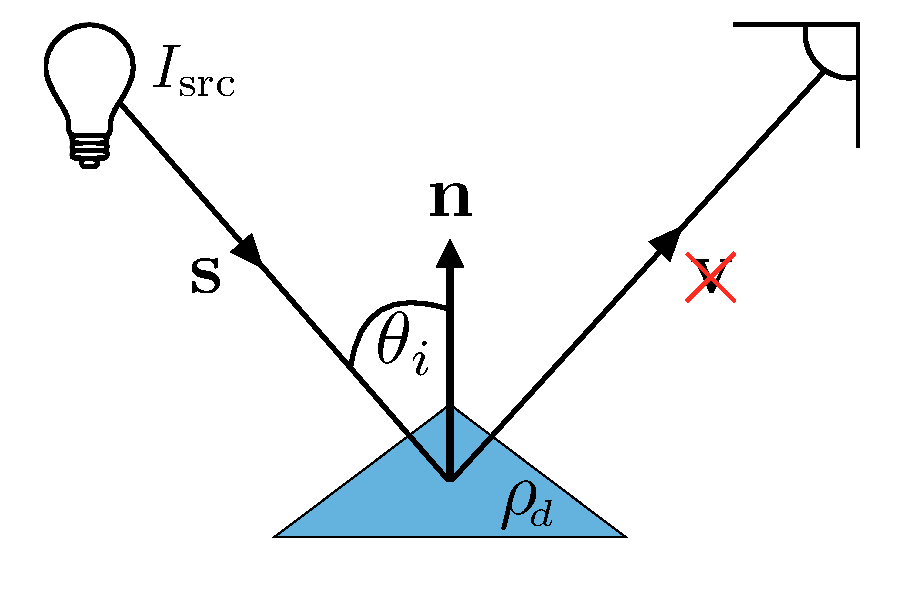
\includegraphics[width=\textwidth]{background/images/lambertian_brdf}
		\caption*{Lambertian BRDF}
	\end{subfigure}
	\caption{The left image shows the general radiance equation for a generic
	         BRDF that is parametrized by the irradiance $(\theta_i, \phi_i)$
	         and radiance $(\theta_r, \theta_r)$ reflecting from the surface. 
	         The right image shows the Lambertian BRDF assuming unit light
	         intensity. Note that the Lambertian BRDF is independent of
	         the viewing direction.}
\label{fig:sfs_brdf_example}
\end{figure}
%%%%%%%%%%%%%%%%%%%%%%%%%%%%%%%%%%%%%%%%
%%%%%%%%%%%%%%%%%%%%%%%%%%%%%%%%%%%%%%%%%%%%%%%%%%%%%%%%%%%%%%%%%%%%%%%%%%%%%%%%
\subsection{SfS Facial Surface Recovery}
%%%%%%%%%%%%%%%%%%%%%%%%%%%%%%%%%%%%%%%%%%%%%%%%%%%%%%%%%%%%%%%%%%%%%%%%%%%%%%%%
%%%%%%%%%%%%%%%%%%%%%%%%%%%%%%%%%%%%%%%%%%%%%%%%%%%%%%%%%%%%%%%%%%%%%%%%%%%%%%%%
